\documentclass[11pt]{article}
\usepackage[utf8]{inputenc}
\usepackage[parfill]{parskip}
\usepackage{graphicx}
\usepackage{enumerate}
\usepackage{amsmath}
\usepackage[title]{appendix}
\usepackage[margin=25mm]{geometry}
\usepackage{amsmath,graphicx,psfrag,pstricks}
\def\n{\noindent}
\usepackage{rotating}
\def\u{\underline}
\usepackage{gensymb}
\def\hs{\hspace}
\newcommand{\thrfor}{.^{\displaystyle .} .}
\newcommand{\bvec}[1]{{\bf #1}}
\usepackage{graphicx}
\usepackage{rotating}
\graphicspath{}
\usepackage{amsmath}
\usepackage{booktabs}
\usepackage{siunitx}
\usepackage{amssymb}
\usepackage[utf8]{inputenc}
\usepackage[justification=centering]{caption}
\usepackage{float}
\renewcommand{\vec}[1]{\mathbf{#1}}
\usepackage{listings}
\usepackage [english]{babel}
\usepackage [autostyle, english = english]{csquotes}
\MakeOuterQuote{"}
\setcounter{tocdepth}{2}


\title{Part IIA Project - GF1: Control Systems - Final Report}
\author{Bailey Brookes | Corpus Christi | bdb31}
\date{\today}

\begin{document}

\maketitle

\begin{abstract}
An evaporator process is to be controlled, with several safety critical parameters and one parameter that determines profitability are to be controller with certain inputs. The system is designed and tested in Simulink with a number of control schemes tested and schemes. The response of each of these schemes is schemes and conclusions and recommendations o the systems to use are made taken into account the performance of the system, the complexity of the implementation  and the cost of implementation 

\end{abstract}

\tableofcontents 

\section{Introduction}
System control is important for a number of response. Process may have to be keep within a certain range to ensure stability and safety. Unstable processes can have dangerous consequences and some variable may want to be maximized/minimize to maximize profitability, minimize wastage or keep costs low. Therefore control systems must be carefully designed and implemented to ensure a system is stable, has predictable responses, and meets the systems requirements.

In this project, an evaporator process is modelled ans controlled in Simulink. The main variable which needs to be controlled is the ‘Product Composition’,  X2, where keeping variations in the composition as small as possible maximizes the profitability of the evaporator, because it minimizes production of out-of-spec product , while minimizing production costs, since it is possible to aim for a composition only a little better than the minimum acceptable one. It is also necessary to operate the evaporator safely, and without damaging the installed equipment. This requires the pressure in the evaporator (P2), and the level of liquid in the separator (L2), to be controlled. To achieve this, several control schemes, such as PI control, gain scheduling and Linear quadratic Regulation, are considered a well as process robustness and the effect of integrator wind-up. These control schemes are compared, and recommendations made on suitable control systems to use. 

A full outline of the project is given in the week 1 handout.

\section{Modelling using Simulink}
In the design of a control system, Simulink is a valuable tool in designing, testing and modelling control systems. The full process can be modeled in Simulink and controllers designed and analyzed. A full report on the modelling of the process can be found in "Part IIA-GF1: Control Systems -First Interim Report" which is attached as an appendix. 

\section{Elaborating the Model and Closing the L2 Loop}
Simulink can be used to model the process more accurately by the addition of lags caused by servos in the process. Control can be added to certain outputs to ensure a desired set point is reached in a particular way. A full report on elaborating the model and controlling the separator level L2 can be found in "Part IIA - GF1: Control Systems - Second Interim Report". Below is a summary of this work.

\begin{itemize}
    \item Two design method for proportional control L2-F2 loop are considered. The heuristic method is simple but lacks any theatrical background. Using the linearised model and bode plot allows for precise control over the phase margin via the choice of gain.
    \item Despite the presence of an integrator in the separator,There is still steady sate error. An integrator forces a zero signal at its input in steady-state, assuming that all signals converge. In a conventional feedback block diagram where the plant contains an integrator but not the controller, this property ensures zero steady state error for a reference step input but not for a load disturbance step input. So integrator control was designed and added.
    \item To improve the model so that it represents the real-world process better, constraints on certain input variables are added to cause saturation when values become too large or small. Control with this limits is not affected.
\end{itemize}

\section{Further Control}

\subsection{Controlling Operating Pressure P2}
The controller for P2, using F200 as the control variable, is designed in the same way as that for L2, which is detailed in the week 2 handout and second interim report. The requirements are also the same: For proportional control only ensure the phase margin is 45\degree and then introduce a phase delay using integral control to result in a phase margin of 40\degree. This is achieved with a proportional gain of $-803.5$ and integral gain of $\frac{-803.5}{12}$.

\subsubsection{Integrator wind-up}
Integral control has one risk associated with it: an integrator can continue to integrate, even though the actual control variable which it determines has become saturated and can no longer increase. This is termed integrator wind-up and is usually the result of a large, long lasting error signal of the same sign. When the error finally reduces to zero there is still a large control signal due to the integrator output, causing the error to become large in the opposite direction since it takes a long time for the integrator output to come back to zero. Several schemes for this exist such as back-calculation and clamping, both of which can be implemented in Simulinks PID block.

In this process, clamping is used as the integrator wind  protection. Clamping, also known as conditional integration, switches off the integration when the control is far from steady state, meaning integral action is only used when certain conditions are fulfilled, otherwise the integral term is kept constant,'clamping' the value. Clamping works by switching off the integration when the controller reaches saturation and the integrator update is such that it causes the control signal to become more saturated, but is kept on if update would move it away from saturation. Upper and lower saturation values are chosen to keep the values which it controls within the operating limits and Simulink implements the control,within its own PID block, which can be expanded to see how it works. The advantage of this over back calculation is that the back calculation gain $K_b$ does not need to be designed, but clamping is harder to implement in the real world as it requires logic circuits to determine how the integral update would effect the error and to turn integration off. 

Figure \ref{fig:P2_Windup} shows the effect of integrator wind up in the control of P2 when a pulse of 20\% of X1 acts for 100 minutes. To stop this wind-up from occurring, some clamping was implemented in all the PID controllers using saturation values that keep all variables within there operating limits. The result of adding integrator wind-up protection is also shown. It's clear from the plot that without protection, P2 fails to reach the operating point after the pulse due to integrator wind up, a problem which is solve by the addition of clamping, which does reach the desired operating point.

More on integrator wind-up and protection schemes can be found in \cite{windup}.

\subsection{Controlling Product Composition X2}
For controlling X2 with steam pressure P100 as the control variable, the "Ziger-Nichols" design method is used. This method is outlined in the week 3 handout, a results in a simple PI controller with proportional gain 4.41 and integral gain 0.3. 

In introducing additional controllers, it is important to check other loops as closing other loops may affect there behaviour. For example, the L2 loop changes marginally with closing the X2 and P2 loops but not substantially so that the controller gains need to be redesigned. The new phase margin of L2 is around 30, not the expected decrease to 10-15.

\subsection{Process Robustness}
Real processes never behave exactly as there are modelled, so it is important to investigate the robustness of the process. Here we investigate changes in the Mass, UA2 and $\rho A$ by varying the parameters and plotting the response of different outputs. We want the response of key outputs (L2, P2 and X2), to not vary much with changes in parameter values. The following test where conducted without integrator wind up protection.

\subsubsection{The effect on L2}
Figure \ref{fig:L2} shows that it is robust when the parameters vary. While to transient response varies slightly, they all have a settling time around 40 minutes.

\subsubsection{The effect on X2}
Figure \ref{fig:X2} shows that X2 has some robustness, with settling times varying from 30-100minutes and varying transient response. The parameter UA2 has the most effect on the response, which changes most left to right.

\subsubsection{The effect on P2}
Figure \ref{fig:P2} shows that P2 without integrator wind up protecting has robustness for changes in M and $\rhoA$, but not for changing UA2 with the process being unstable at lower values and having varying settling times at high values. This is undesirable as it means the response of P2 can vary drastically, and P2 is a key parameters as too higher pressure can be unsafe if the evaporator is only rated up to a certain operating pressure. IF it grows without bound or to a too high value, the process could fail. So some production needs to be added to improve robustness.

\subsubsection{The effect of integrator wind up protection}
Process robust for P2 is dramatically improved when integrator wind up protection is added as shown in Figure \ref{fig:p2_robust}. This is expected as this stops wind up which can cause the response to grow, saturated and overshoot. Integrator windup up protection on the L2 and X2 PI controllers also improves there robustness to almost identical responses, shown in Figures \ref{fig:l2_robust} and \ref{fig:x2_robust} respectively. This highlights another advantage of wind up protection, the robustness is increased dramatically so it is highly recommended that the final design has integrator wind up protection. 

\section{Week 4 Plan}
Week 4 involved several task to be spit between the team: testing of current control methods, gain scheduling control and multivariate control. The first 2 task where each given to one person, taking on a task each. The multivariate control, being the most complicated, was given to two others. Once everyone had done there task, everyone was brought back to together to exchange results and discuss conclusions drawn from them.

\begin{figure}[H]
    \centering
    \includegraphics[scale = 0.4]{plan.png}
    \caption{Gantt cahrt of the teams week 4 plan}
    \label{fig:my_label}
\end{figure}

The team reasonable for task 3 found out task 4 (a different form of multivariate control) didn't need to be done as there solution (LQR control, see later) worked adequately for the requirements. Therefore task 4 (manual multivariate control, see later) was not done.

\section{Testing Changes of Operating Point}
It is desirable to have reliable, consistent behaviour at a number of operating points for economic reasons like increasing or decreasing the rate solvent is evaporated demanding on demand for the product. The controller designed so far have only been designed for one specified operating pint given in the handout. However it is important to investigate if this control is suitable and if not, what is the best method of adapting this control. 'Best' can either mean the best control when money and difficult of implementation is no object, or simple control that is cheap and easy to implement and is adequate for the design specifications.

Product Concentration (X2) was chosen to test the suitable of control and its response is shown in Figure \ref{fig:Non_set} at a set point of 25\%. This response has an overshoot of around 30\% and a settling time of 50 minutes. If this is now compared to the response at 15\% and 35\% set-points, also shown in Figure \ref{fig:Non_set}, we can see the response is drastically different, with overshoots of 14\% and 3\% and settling times of 80 and 100 minutes respectively. Figure \ref{fig:X2_stairs} also shows the response of X2 to steadily increasing and decreasing set points. Now while X2 always reaches the desired set point in under 100 minutes, its initial response when the set point changes varies. Depending on the design criteria set this may be acceptable, but if consistent response are desired at all operating points, alternative forms of control must be considered. We look at 2: Gain scheduling and multivariate control.

\section{Improvements from testing}

\subsection{Gain scheduling}
In the single input, single output control, the proportional and integral control gains are fixed and don't change with operating point. Because the Process is no linear, this causes the response to change at low and high values of X2, so a single controller is unsuitable. A simple method to combat this is the use different controllers at different operating points, using the value of X2 to choose the controller to use. To implement gain scheduling we require:

\begin{itemize}

    \item An operating range, defined as a set of ranges within which the values of relevant system parameters remain during operation. We will assume X2 varies from 15\% to 35\%.

    \item Some measurable variables that indicate where in the operating range the system is at a given time. These signals are the scheduling variables. This is the production concentration X2.

    \item A gain schedule, which is a  data table that return the appropriate controller gains for given values of the scheduling variables. For the process, this changes the value of the proportional and integral gains.

\end{itemize}

The final design of the X2 gain scheduling control is shown in Figure BLANK.

Figure \ref{fig:X2_Stairs_schedua} shows the response now with gain scheduling. This shows a more consistent response at each set point, with overshoot and oscillation down to the final value, like it is at 25\%. This can also been seen at the 15\% and 25\% set points as shown in Figure \ref{fig:GS}.

\subsection{Multivariate Control}
Up until now, single input single output control has been used. While simple, it ignores the fact that several variables may effect one output, and just focuses on one input. In the evaporator process, there is considerable interaction between the three controlled variables X2, P2 and L2. Better control may therefore be possible by implementing a multivariate controller which controls all three variables in a coordinated way, rather than three separate single-loop controllers. The way to do this is to use state feedback. One approach would be to get the linearised state space module of the system and then to place the poles manually using a proportion gain controller with matrix of gains K. Pole placement must ensure that the poles placed  are “much faster” than the dominant 2nd order behavior of the process. While this allows the system response to be tuned to specif requirements, getting the optimum controller would have to be done manually by trial and error. Optimization could be done by making an appropriate cost function and then minimizing that. An method of design that does this is Linear Quadratic regulation (LQR).

\subsubsection{Linear Quadratic Regulator}
An alternative approach is to place poles to optimize the following cost function:

\[J_{LQR} = \int_0^\infty \bold{x}^T(t)Q\bold{x}(t) + \bold{u}^T(t)R\bold{u}(t)\hspace{0.5em} dt\]

where $\bold{x}^T(t)Q\bold{x}(t)$x is the state cost (the seriousness of an error) with weights in $Q$, and $\bold{u}^T(t)R\bold{u}(t)$ is the control cost( the difficulty of control of each input)  with weights in $R$. Q and R are diagonal matrices with each element being a weight corresponding to an state or input for $Q$ and $R$ respectively. $\rho$ is the relative weighting between state  and control cost, with  a high $\rho$ corresponding to a higher control cost.

\[
Q = 
\begin{bmatrix}
	q_{11} &  		&  		& 		\\
           & q_{22} &  		& 		\\
           & 		&\ddots & 		\\
           & 		&  		& q_{nn}
\end{bmatrix}
\hspace{2cm}
R = \rho
\begin{bmatrix}
	r_{11} &  		&  		& 		\\
           & r_{22} &  		& 		\\
           & 		&\ddots & 		\\
           & 		&  		& r_{mm}
\end{bmatrix}
\]

The state feedback matrix is then found from $\bold{\hat{u}} = −BR^{−1}P\bold{\hat{x}}$, giving $K = BR^{-}P$. $P$ is found by solving the algebraic Riccati equation:

\[
0 = P A + A^T P - PBR^{-1} B^TP + Q
\]


All this can be done by using Matlabs \texttt{lqr}  function: \texttt{K = lqr(A, B, Q, R)}, where A and B are the state space matrices of the linearised version of the process. 

What LQR does is assign importance values to each state and input so the controller is more sensitive to certain states  but less so to others. This means a state space controller can create an optimum controller easily, with only the weights of $Q$ and $R$ needing to be specified. A common way to chose the weights is to us Bryson’s rule \cite{LQR} which normalizes the values depending on the maximum allowable value of each input. Further weighting can be applied to vary the amount each input contributes to cost, but for testing they were all weighted equally:

\[ q_{nn} = \frac{1}{x_{n,max}^2} \hspace{1cm} r_{mm} = \frac{1}{u_{n,max}^2}\]

The parameter $\rho$ can also the varied to further optimize the controller, being chosen by running the controller for a number of different $\rho$ and choosing the optimum. For this system, the value is 1.

\subsubsection{Proportional Control}
With control inputs $\bold{u} = [F2, P100, F200]^T$ an states $\bold{x} = [L2, X2, P2]^T$, and therefore $\bold{\hat{u}} = [F2 -F2_{nom}, P100 - P100_{nom}, F200 - F200_{nom}]^T$ an outputs $\bold{\hat{x}} = [L2 - L2_{set}, X2 - X2_{set}, P2 - P2_{set}]$ the $Q$ and $R$ matrices are:

\[
Q = 
\begin{bmatrix}
	\frac{1}{1} &  		&  		& 		\\
           & \frac{1}{9} &  		& 		\\
           & 		&  		& \frac{1}{50.5^2}
\end{bmatrix}
\hspace{2cm}
R = \rho
\begin{bmatrix}
	\frac{1}{4} &  		&  		& 		\\
           & \frac{1}{194.7^2} &  		& 		\\
           & 		&  		& \frac{1}{208^2}
\end{bmatrix}
\]

X2 did not have a saturation value, so a maximum product concentration error tolerance of 3\% was chosen. 

The gain matrix was implemented by having three controllers, one for each control input, with each
controller having a proportional gain for each output error. Each proportional gain was set directly from the resulting gain matrix K calculated by Matlab.

The response of the system to changing set points was as expected; errors died away and the system
reached the new set points, but changing inputs resulted in steady state errors. This is shown in Figure \ref{fig:LQR P}


\subsubsection{PI Control}
To include integral control and remove steady state errors, the only change in the analysis is to change the matrices A and B so that they include integral control. That is:

\[ 
\Tilde{A} = 
\begin{bmatrix}
    A & 0\\
    I & 0
\end{bmatrix}
\hspace{1cm}
\Tilde{B} =
\begin{bmatrix}
    B \\ 0
\end{bmatrix}
\]

Where $I$ incorporates the integral control. 

The new $Q$ weights to the three new outputs had to be calculated, which required setting
a maximum integrated error value. This is done by using the worst response which is approximated as a pulse from
zero to saturation of time $t_{max}$, selected to be 20 minutes for each error, and the area of
the pulse calculated, as per Figure \ref{fig:area}. For our system that was $20\times30 = 60$.

\begin{figure}[H]
    \centering
    \includegraphics[scale = 0.5]{thatthing.png}
    \caption{an integral action response (left), approximating the maximum integral action response
    (right)}
    \label{fig:area}
\end{figure}

The Q matrix was updated, and the expanded K matrix calculated for several values of $\rho$.  The full LQR controller then is shown in Figure \ref{fig:LQR Controller}. The downside of LQR control is clearly seen: There is a lot of modules that must be implemented and the complexity of the model increase by more states are inputs are added to the design as well as the type of control (the addition of differential control would add other 9 gains to be calculated). The advantages of LQR is that it is the optimum controller at all operating points. 

The range of $\rho$ values tested was done according to $\log \rho$; for example, when $\log \rho = −1$, state
cost is 10 times larger than control cost. As expected with integral control, the system responded
well to step input changes. It was noted that the system responded best to set point changes when
$\log \rho \leq 0$, and the system responded best to input changes when $\log \rho \geq 0$, so $\log \rho = 0$ was chosen to allow the system to handle both. Further testing was done with random disturbances to input
and set points as shown in Figure \ref{fig:LQR Random} the system was stable for all disturbances.

\subsection{Comparing gain scheduling and LQR}
Gain scheduling and LQR both try to overcome the problem of inconsistent behavior of the process at different set points but in different ways. Gain scheduling is still a single input, single output (SISO) controller but uses the output to change the controller gains according to where the process is at. LQR however is a multi input single output (MISO) controller that uses a cost function to optimize its control at all set points. 

Gain scheduling is the similar method, with only some look up tables/functions need to be added to change the controller gain. It can be easily expanded to include more set points or to vary smoothly between gains as the set points change. However it is not the optimum controller at all set points, which LQR is.

LQR is the optimum controller at all set points and is easy to design, with only the importance weights in $Q$ and $R$ needing to be specified, with accepted methods of choosing them available. However, it is more complex to implement in practice and grows in complexity faster the more forms of control used and the more inputs used to control. 

The choice then of which form of control to used depends on the requirements of the process. If the response must be identical at all set points and parameters have tight constraints, then LQR would be the control scheme to use. If however the settling time or stability is all that required, then simple gain scheduling with anti wind up schemes would be suitable. Of course the same form of control doesn't need to be used throughout. Operating pressure and separator level for example is a safety critical parameter that must have stable predictable behaviour, so LQR control would be beneficial. However production composition are not safety critical but is variable of interest from a profitability standpoint process, so a decision of cost of implement ion of a scheme vs its resulting profitability must be done to choose an appropriate scheme. Gain scheduling for example can be used to ensure a similar settling time for all set points, with the complexity of the gain scheduling scheme (number of different gains, linear interpolation between them) be varying according to desired performance. Alternatively LQR would give optimal performance but the cost may outweigh the resulting profit.

\section{Conclusions}

\paragraph{Further Control}
\begin{itemize}
    \item SISO control is added to X2 and P2 to meet similar requirement that set on L2 in the first week
    \item Integrator wind up is an issue where an integrator keeps integrating even when its output has reached saturation. This can cause overshoots and instability, as well as loss in robustness at different parameters. By adding clamping as integrator wind up protection, the response of not only P2 but X2 and L2 is improved dramatically.
    \item Without integral control, the system is fairly robust except P2 when UA2 is varied. Since the operating pressure is safety critical, robustness must be improved, The addition of integrator wind up protection  dramatically increases the robustness of all parameters.
\end{itemize}

\paragraph{Advanced control}
\begin{itemize}
    \item Testing revealed that parameters have different responses at different set points. Since it is desirable for the process to act a number of set points for economic reasons, this must be fixed. To method where considered to do this: Gain scheduling at LQR.
    \item Gain Schelling use the parameter that it controls to decide what controller gains to use. This allows to control to vary depending on parameters set point. The idea is that the system response the same at a number of set points, a desirable property for economic reasons. In our process, simple gain scheduling which changes controller gains at 20 and 30\% effectively gives similar responses at 15\%, 35\% and varying set point. Gain scheduling is simple to implement and ca be further improved by additional controller gains and smoothly varying between them.
    \item A Linear Quadratic Regular (LQR) gives optimal control by minimizing a cost function by varying state and input costs, relating to how hard they are to control/how much they effect the output. This is simple to design but is complex to implement but does give optimal control at all set points.
    \item It is possible to combine LQR and gain scheduling control depending on the system requirements. For example, for a safety critical parameter such as operating pressure P2 and speatro level L2, LQR would ensure optimal control at all safe operating pressures and would give much ore similar response than gain scheduling. Product composition X2 is less saftey critical but does affect the profitability of the system, so a trade off between cost of implementation of control vs resulting profit would need to be considered before decing a suitable control scheme.
    \item To fully decide the best control system, the exact requirements of the system and its parameters would need to be given to decide if simple single input single output, integrator wind up protection, gain scheduling or LQR or a combination of these is needed, with the overall goal of minimizing wastage/cost.
\end{itemize}

\paragraph{Suggestions of Further Work}

\begin{itemize}
    \item Further investigation into integrator wind up protection techniques would give insight into there designing and easy of implementation, rather than using Simulinks built in clamping which may be difficult to implement.
    \item Gain Schelling could be further improved with more controller gains and some linear interpolation between schemes.
    \item LQR at present uses 3 control inputs. Further investigation could be carried out to see if more would further optimize the control or if less would still give acceptable control while decreasing the complexity of implementation.
    \item A investigation of cost of implementation vs resulting improvement in profitability/safety should be carried out to see what is the most suitable control scheme for each variable.
\end{itemize}

\begin{thebibliography}{9}
\bibitem{windup} 
K. Åström, T. Hägglund. 
\textit{Advanced PID Control}. 
ISA, Research Triangle Park, NC, August 2005.
 
\bibitem{LQR} 
R. M. Murray. 
\textit{Lecture 2 – LQR Control}.
California Institute of Technology 2006
 
\bibitem{Feedback Control Systems} 
Feedback Control Systems \newline
\texttt{https://ocw.mit.edu/courses/aeronautics-and-astronautics/16-30-feedback
\newline
-control-systems-fall-2010/lecture-notes/MIT16\_30F10\_lec12.pdf}

\bibitem{Digby}
MIT OpenCourseWare

\end{thebibliography}

\appendix
\section{Plots and Figures}

\subsection{Integrator wind-up }

\begin{figure}[H]
    \centering
    \includegraphics[scale=0.35]{P2_Windup.jpg}
    \caption{Response of operating pressure P2 with and without clamping to a pulse on X1}
    \label{fig:P2_Windup}
\end{figure}

\subsection{Process Robustness}

\begin{figure}[H]
    \centering
    \includegraphics[scale=0.25,angle = 90]{L2.jpg}
    \caption{Response of separator level L2 for different process parameters}
    \label{fig:L2}
\end{figure}

\begin{figure}[H]
    \centering
    \includegraphics[scale=0.25,angle = 90]{X2.jpg}
    \caption{Response of product composition X2 for different process parameters}
    \label{fig:X2}
\end{figure}

\begin{figure}[H]
    \centering
    \includegraphics[scale=0.25,angle = 90]{P2.jpg}
    \caption{Response of operating pressure P2 for different process parameters}
    \label{fig:P2}
\end{figure}

\begin{figure}[H]
    \centering
    \includegraphics[scale=0.25,angle = 90]{p2_robust.jpg}
    \caption{Response of operating pressure P2 for different process parameters with integrator wind up protection}
    \label{fig:p2_robust}
\end{figure}

\begin{figure}[H]
    \centering
    \includegraphics[scale=0.25,angle = 90]{l2_robust.jpg}
    \caption{Response of separator level L2 for different process parameters with integrator wind up protection}
    \label{fig:l2_robust}
\end{figure}

\begin{figure}[H]
    \centering
    \includegraphics[scale=0.25,angle = 90]{x2_robust.jpg}
    \caption{Response of production composition X2 for different process parameters with integrator wind up protection}
    \label{fig:x2_robust}
\end{figure}

\subsection{Testing Changes of Operating Point}

\begin{figure}[H]
    \centering
    \includegraphics[scale = 0.23,angle =90]{Non_set.jpg}
    \caption{Response of product composition X2 at a 15\%, 25\% and 35\% set points}
    \label{fig:Non_set}
\end{figure}

\begin{figure}[H]
    \centering
    \includegraphics[scale = 0.25,angle =90]{Stair_Change_test.jpg}
    \caption{Response of product composition X2 at varying set points}
    \label{fig:X2_Stairs}
\end{figure}

\subsection{Gain Scheduling}

\begin{figure}[H]
    \centering
    \includegraphics[scale = 0.23,angle =90]{GS_set.jpg}
    \caption{Response of product composition X2 at a 15\%, 25\% and 35\% set points with gain scheduling}
    \label{fig:GS}
\end{figure}

\begin{figure}[H]
    \centering
    \includegraphics[scale = 0.25,angle =90]{Stair_Change.jpg}
    \caption{Response of product composition X2 at varying set points with gain scheduling}
    \label{fig:X2_Stairs_schedua}
\end{figure}

\subsection{Multivariate Control}

\begin{figure}[H]
    \centering
    \includegraphics[scale = 1,angle = 90]{Picture1.png}
    \caption{System response using LQR with proportional control}
    \label{fig:LQR P}
\end{figure}

\begin{figure}[H]
    \centering
    \includegraphics[scale = 0.25]{ControllerFinal.png}
    \caption{LQR controller for the process}
    \label{fig:LQR Controller}
\end{figure}

\begin{figure}[H]
    \centering
    \includegraphics[scale = 0.8]{LQR_PI.png}
    \caption{System response to random step changes in step points using LQR with PI control}
    \label{fig:LQR Random}
\end{figure}

\section{First Interim Report}
\subsection{Subsystems}
\subsubsection{Evaporator}
Due to the evaporator having derivatives in its equation, design is done by first taking Laplace transforms of the equations, revealing that there are two integrators. Therefore overall the system has 3 states, one in the separator and two in the condenser.

To test the evaporator subsystem, step inputs are placed at all inputs and outputs measured after a certain simulation time. This simulation time is found by considering the two negative feedback loops which both contain integrators. The negative feedback makes the system stable, and constant F1 and F2 make the system stable as product blocks act as gains. Using this gains the time constants for each loop can be found by considering each loop as a integrator with gain $k$ and negative feedback. The transfer function for such a system is $G(s) = \frac{s}{s+k}$ with pole $-k$  and time constant $\frac{1}{k}$. So for the X2 and P2 loops:

\begin{itemize}
\item X2 Loop has loop gain (pole) $0.05$ and a time constant of 20 
\item P2 has loop gain (pole) $2.5527 \times 10^{-4}$ and time constant $3917.42$ 
\end{itemize} 

So the simulation should be run for a duration a couple times bigger than the largest time constant. The plots of some of the outputs are show in Figures \ref{P2}, \ref{X2} and \ref{F4}, showing the model is stable.

\subsubsubsection{Linearising the Evaporator}
Simulink allows non linear models, such as the evaporator, to be linearised using \texttt{linmod}. This gives the state space model of the linearises system, which is:

\[
A = 
\begin{bmatrix}
-0.05 & 0 \\
-0.0001 & -0.0003
\end{bmatrix}
\hspace{1cm}
B = 
\begin{bmatrix}
0.0500 & 0.0500 & -1.2500 & 0 & 0 & 0\\
-0.0380 & 0 & 0 & -0.2500 & 0.0005 & 0.0065
\end{bmatrix}
\]
\[
C = 
\begin{bmatrix}
    1.0000&         0\\
         0&    1.0000\\
         0&    0.5070\\
    0.3126&    0.5616\\
   -0.0006&   -0.0010\\

\end{bmatrix}
\hspace{2cm}
D = 
\begin{bmatrix}
0&         0&         0&         0&         0&         0\\
0&         0&         0&         0&         0&         0\\
0&         0&         0&         0&         0&         0\\
0&         0&         0&         0&         0&         0\\
-0.1520 &        0&         0&         0&    0.0018&    0.0260

\end{bmatrix}
\]

The eigenvalues of A gives the poles of the linearised system, which are -0.0003 and -0.05. This gives us an additional two checks to the model: 
\begin{enumerate}
\item These poles should correspond to the time constants calculated before. Time constants for these two poles are 3333.33 and 20, with the difference between the larger value down to rounding errors in matlab.
\item Changing F1 by a factor of 10 should make the P2 loop 10 times faster, so the pole (eigenvalue should be one tenth the size. Both the simulink and analytically shows that this is the case, with the system having time constant 33333.33 in simulink and 39174.2077 analytically.
\end{enumerate}

\subsubsection{Condenser and Steam Jacket}
Both the condenser and the steam jacket where designed directly from there equations given in the handout and these systems are shown in Figures \ref{condenser} and \ref{steamjacket} respectively. Complete models of the separator and evaporator depicted in the handout are omitted from the appendix for conciseness.

\subsubsection{Whole Process}
\subsubsection{Test Results}
Testing and debugging revealed one floor in the initial design, that divisor blocks had been used wrong in the condenser, affecting output to all other subsystems. Once the ports had been switch round for these blocks throughout the system, the process's nominal values where reached. 

\subsubsection{Trim Results}
Another method of testing the systems steady state is the trim function in simulink. A trim/equilibrium point is a point in the parameter space of a dynamic system at which the system is in a steady state. That is, when the system's state derivatives equal zero. For this model, these points should be the same as the nominal values given in the handout, with some rounding error. These results from the trim function in simulink are tabulated below.
\begin{table}[H]
\centering
\label{my-label}
\begin{tabular}{|cc|}
\hline
Output & Value    \\ \hline
X2     & 25       \\
P2     & 50.5053  \\
T2     & 84.6088  \\
F4     & 8        \\
F5     & 8        \\
Q200   & 308.0002 \\
T201   & 46.1539  \\
T100   & 119.9449 \\
Q100   & 339.2263 \\
F100   & 9.2685   \\
L2     & 0        \\ \hline
\end{tabular}
\caption{Trim analysis results}
\end{table}

\subsection{First Interim Report Appendix}
\subsubsection{Plots of the evaporator response}

\begin{figure}[H]
\centering	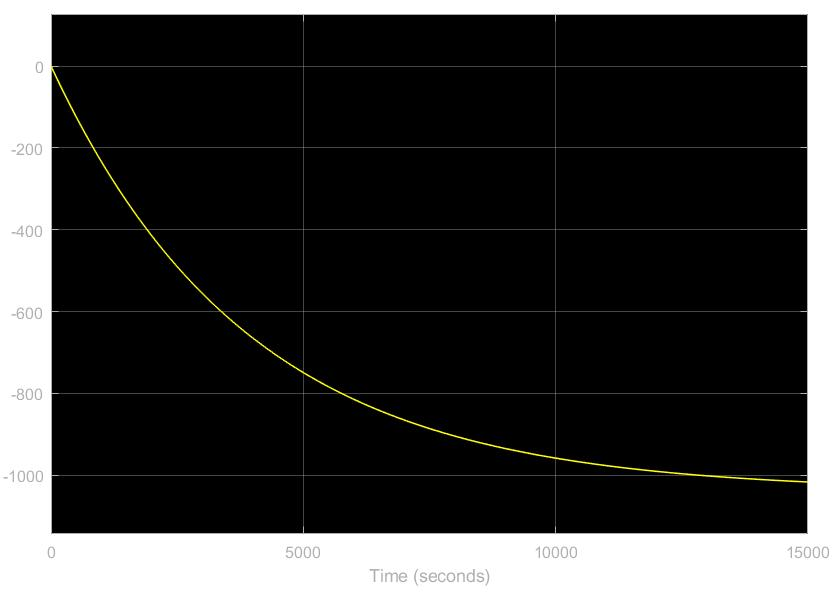
\includegraphics[scale = 0.4]
{P2_15000}
\caption{Response of P2}
\label{P2}
\end{figure}

\begin{figure}[H]
\centering	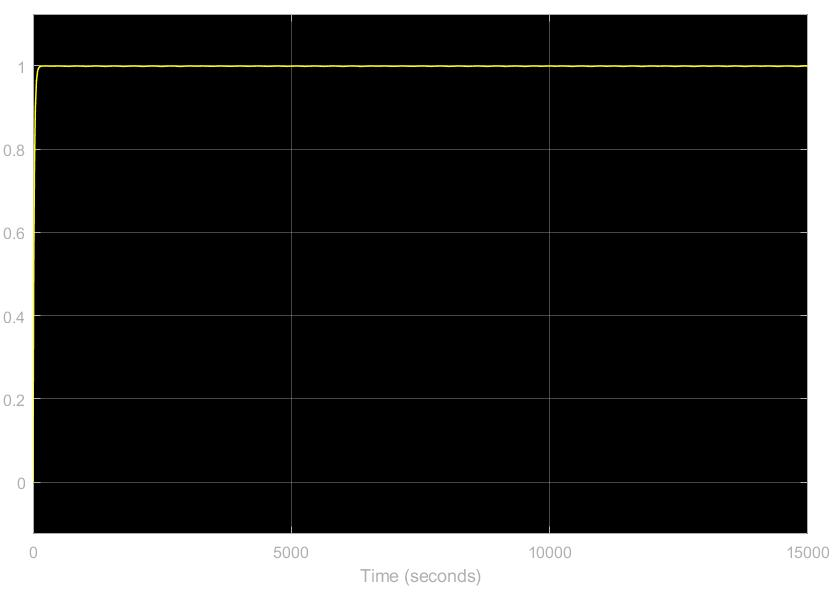
\includegraphics[scale = 0.4]
{X2_15000}
\caption{Response of X2, which is much faster than that of P2, as in seen by the very sharp rise at the start}
\label{X2}
\end{figure}

\begin{figure}[H]
\centering	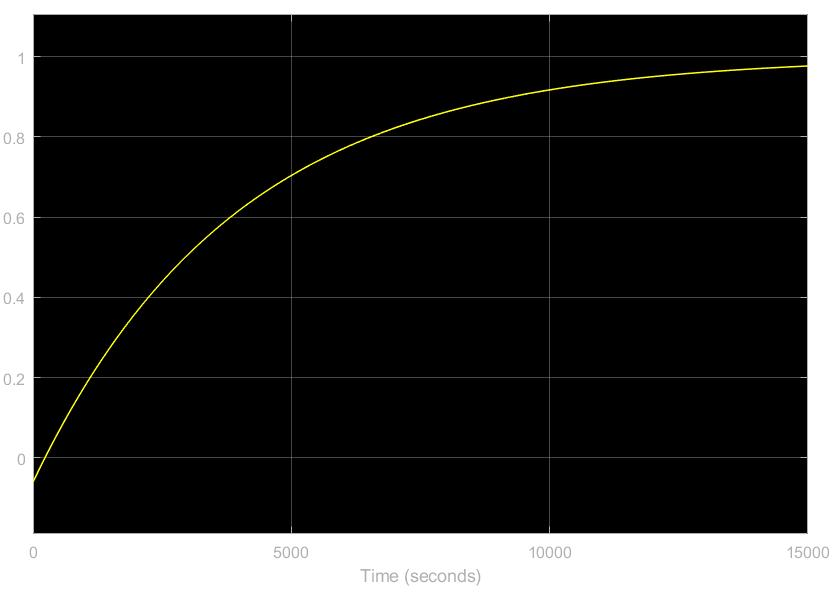
\includegraphics[scale = 0.4]
{F4_15000}
\caption{Response of F4}
\label{F4}
\end{figure}

\subsubsection{Subsystems}

\begin{figure}[H]
\centering	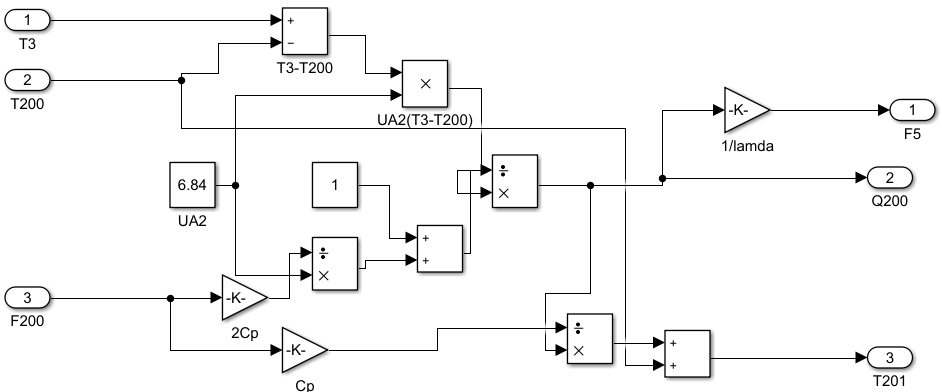
\includegraphics[scale = 0.8]
{condenser}
\caption{Condenser Model}
\label{condenser}
\end{figure}

\begin{figure}[H]
\centering	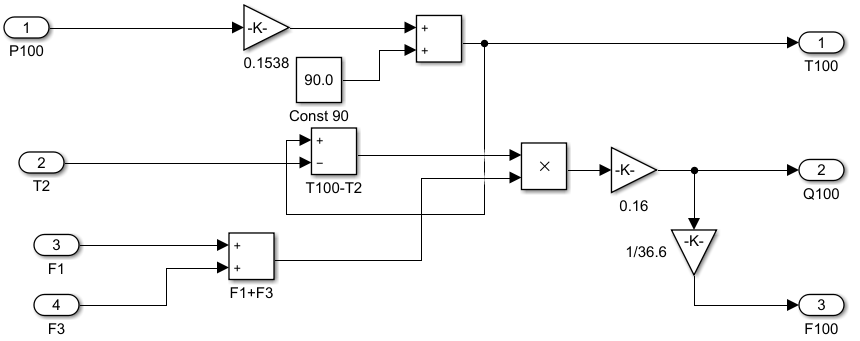
\includegraphics[scale = 0.8]{steamjacket}
\caption{Steam Jacket Model}
\label{steamjacket}
\end{figure}

\subsubsection{Complete Model}
\begin{figure}[H]
\centering	\includegraphics[scale = 0.5]
{Process}
\caption{Model of entire process}
\label{process}
\end{figure}

\section{Second Interim Report}
\subsection{Controlling the separator level}

\subsubsection{Proportional Control}

\subsubsubsection{Heuristic Method}
By adding a slider gain to provide negative feedback and a step input to provide the L2 set-point, such as that show in the handout, trial and error can be used to get the response of the F2-L2 loop to have a 50\% overshoot. The gain that achieves this is -48 and is shown in Figure \ref{L2_man}.

The effect of a $\pm10\%$ change in set point is shown in Figure \ref{L2_setpoints}.These response are the same response but mirrored about the 1m nominal set-point, and both give under/overshoot of 50\% as required.

The effect of a $\pm10\%$ change in the flow rate F1 is shown in Figure \ref{F2_setpoints}. Interestingly, even though the separator acts like an integrator, there is still steady state error when F1 is change. This is discussed later in the report and fixed with a proportional integral (PI) control.

\subsubsubsection{Theoretical Method}
The bode plot for the linearised version of the F2-L2 loop is shown in Figure \ref{OG_bode}. For a phase margin at $45\degree$, the gain plot needs to be raised by 22.9dB which is equivalent to a gain of -13.9. The response of the L2-F2 loop with this gain is shown in Figure \ref{L2_theory} and the bode plot in Figure \ref{-13.9_bode}. 

There is a large difference between the heuristic and theoretical gain, with the theoretical gain giving less overshoot but the required set point and phase margin. The heuristic gain of -48 gives a phase margin of 28\degree, 62\% of what it should be. 

\subsubsection{Proportional and Integral Control}
Changing the F1 flow rate as shown in Figure \ref{F2_setpoints} changes the L2 set-point. Despite an integrator in the separator, there is still steady state error. This is because the integral control removes steady state error by ensuring the sum between set point and curve reaches zero so acts on the error output signal to change the error signal. So feedback is required. The integrator in the separator isn't used in feedback so doesn't remove the steady state error. 

To remove the steady state error an integrator in the control loop is required. The specifications require a phase margin of 40\degree with the integral action in the control, which is the same as having a phase lag of 5\degree at the frequency which gives a phase margin of 45\degree, which is 0.595 rad/s. To calculate T$_i$ in the handout, we solve:

\begin{gather*}
1 - j\frac{1}{0.595T_i} = \tan5\degrees \hspace{1cm} \implies \hspace{1cm} T_i = 19.2
\end{gather*}

The response of this PI controller is shown in Figure \ref{PI_set}, demonstrating that the controller removes the steady state error caused by varying the flow rate F1. The bode plot, which shows that the phase margin is around 40\degree, is shown in Figure \ref{PI_bode}.

\subsection{Constraints on Variables}
Adding constraints on variable makes the model more realistic as many inputs will have maximum or minimum values, be it by design or available input. For example, the feed flow rate can only increase by so much and cannot be negative so is limited to 0 to 20 kg/min.

\subsubsection{Changing X1}
The L2-F2 controller is very robust to step changes in X2. The nominal value is 5\% and the controller behaves well up to 23\% and down to 0\%, which is shown in Figure \ref{X2_Levels}.

\subsubsection{Changing F1}
The L2-F2 controller is much less robust in changes to F1, failing to control the set-point above 12kg/min and below 8kg/min, shown in Figure \ref{F2_Levels}.

\subsection{Second Interim Report Appendix}

\subsubsection{Plots}
\begin{figure} [H]
\centering	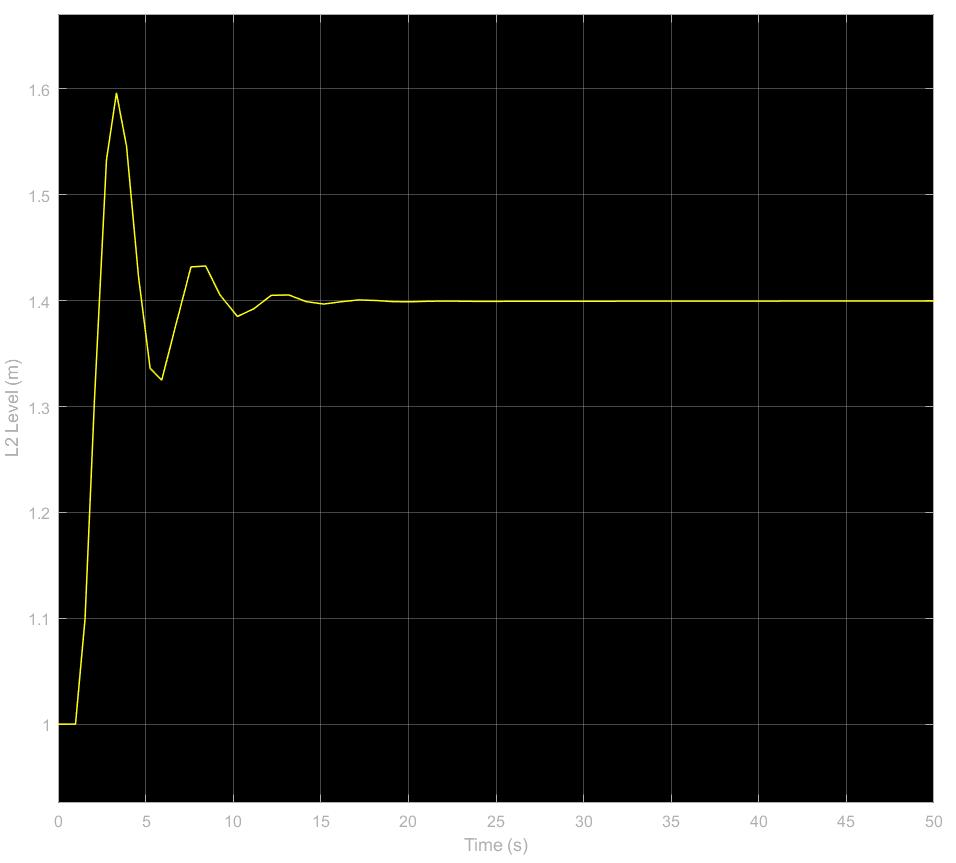
\includegraphics[scale = 0.3]{L2_control_maual}
\caption{Response of the L2-F2 control loop with gain of -48}
\label{L2_man}
\end{figure}

\begin{figure} [H]
\centering	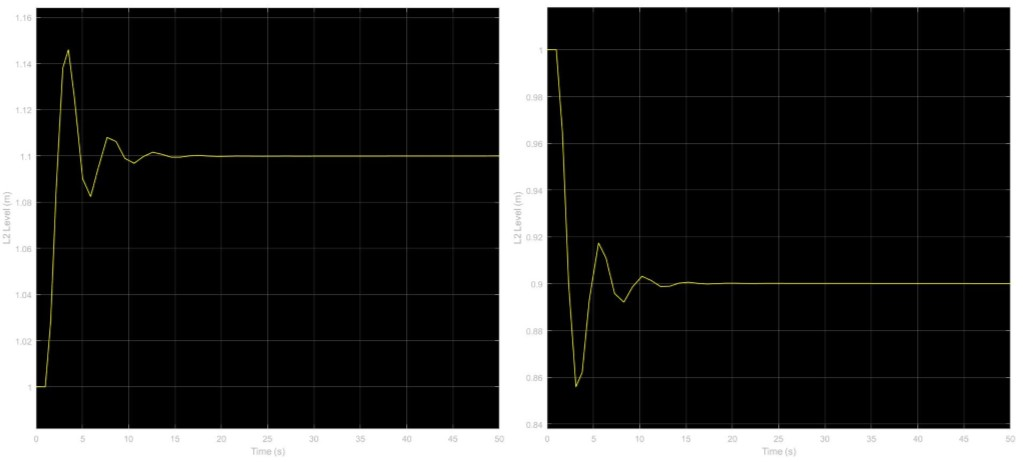
\includegraphics[scale = 0.6]{L2_setpoints}
\caption{Response of the heuristic designed L2-F2 control loop at set-pint of L2 to 1m (left) and 0.9m (Right)}
\label{L2_setpoints}
\end{figure}

\begin{figure} [H]
\centering	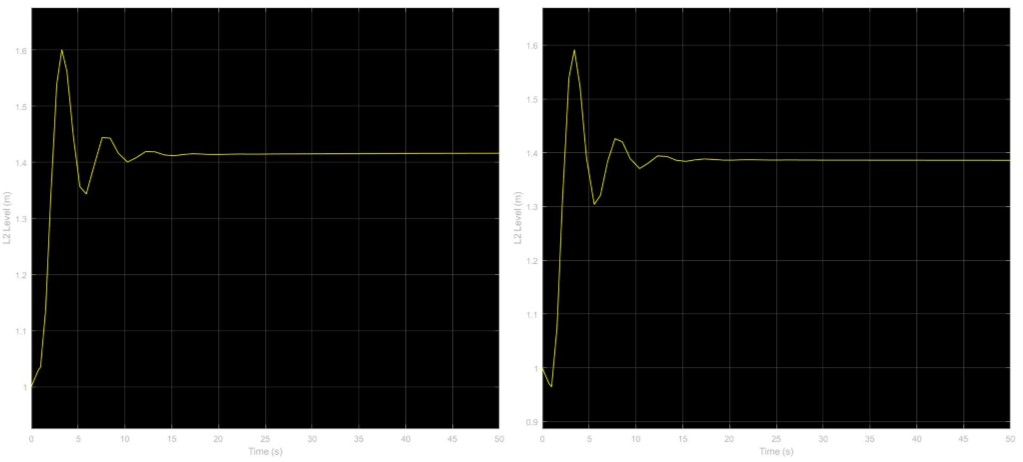
\includegraphics[scale = 0.6]{F2_setpoints}
\caption{Response of the heuristic designed L2-F2 control loop at set-pint of F2 to 11kg/min (left) and 9kg/min (Right)}
\label{F2_setpoints}
\end{figure}

\begin{figure} [H]
\centering	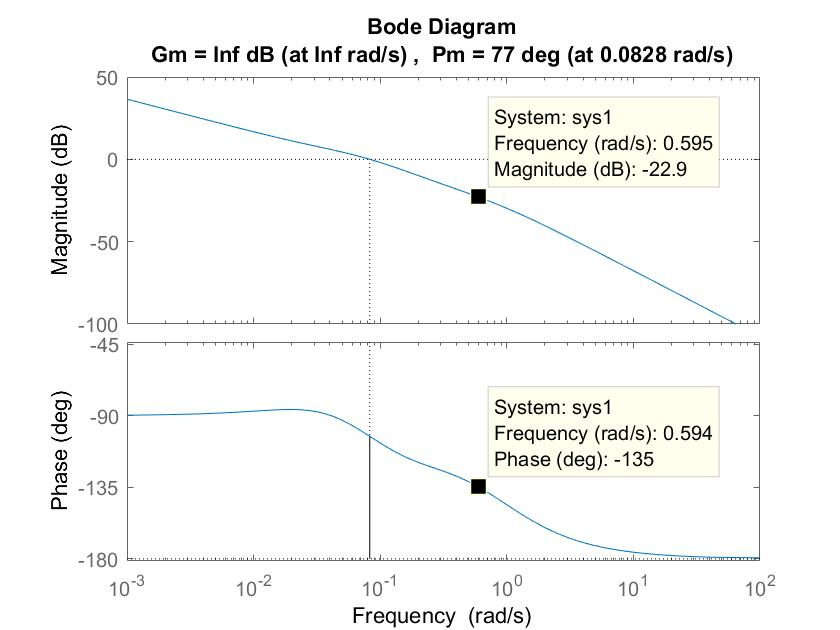
\includegraphics[scale = 0.4]
{L2_Open_bode}
\caption{Bode plot of the open F2-L2 loop}
\label{OG_bode}
\end{figure}

\begin{figure} [H]
\centering	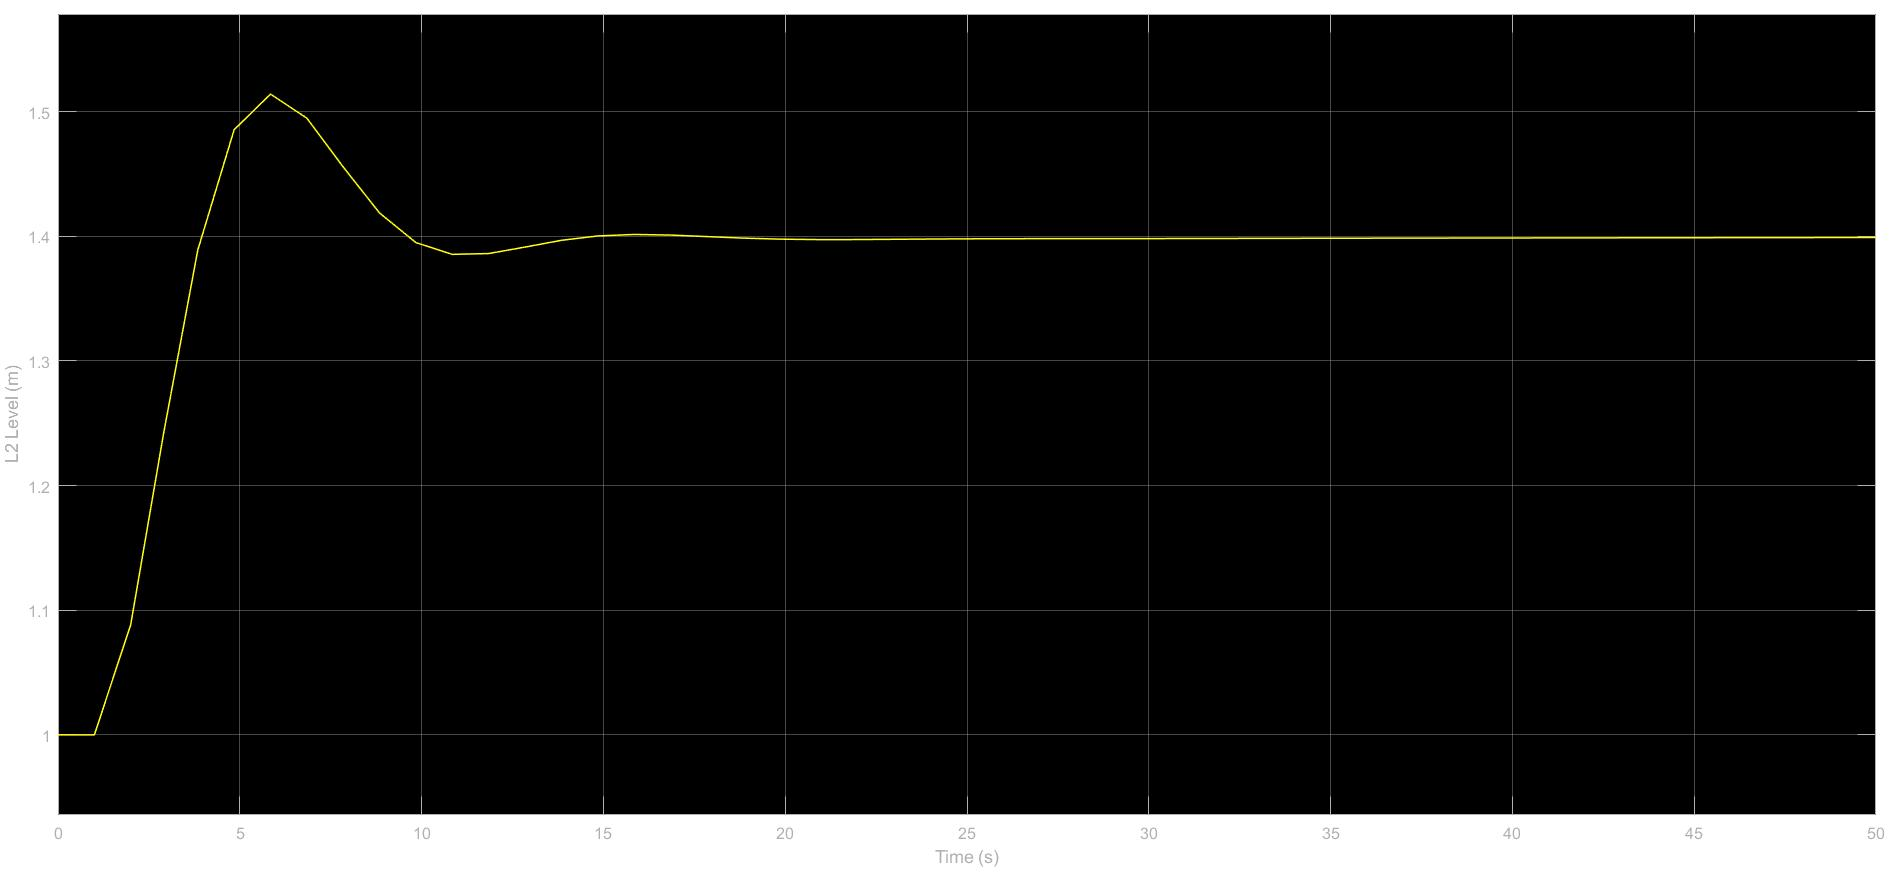
\includegraphics[scale = 0.2]
{L2_theory}
\caption{Response of the L2-F2 control loop with gain of -13.9}
\label{L2_theory}
\end{figure}

\begin{figure} [H]
\centering	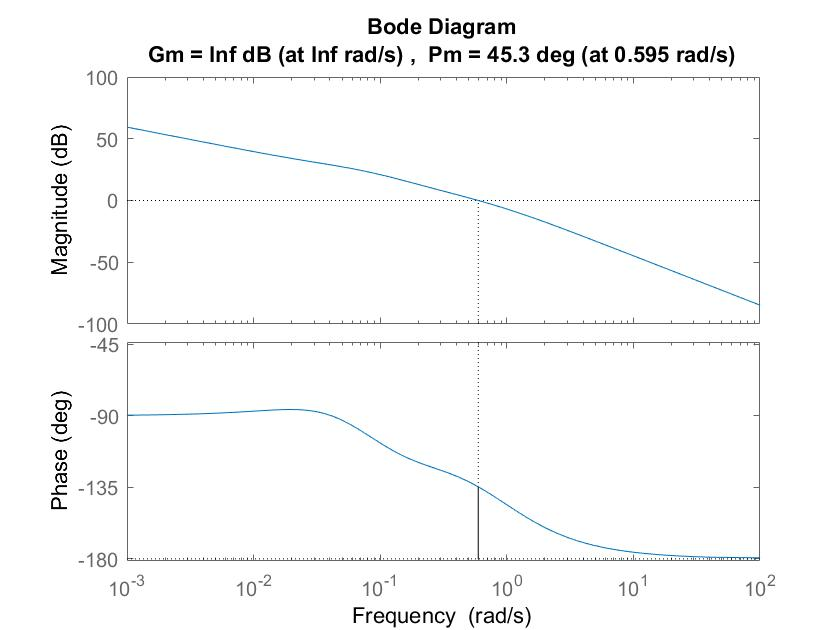
\includegraphics[scale = 0.4]
{L2_139_bode}
\caption{Bode plot of the open F2-L2 loop with gain of -13.9}
\label{-13.9_bode}
\end{figure}

\begin{figure} [H]
\centering	\includegraphics[scale = 0.6]
{PI_set}
\caption{Response of the L2-F2 control loop with PI control}
\label{PI_set}
\end{figure}

\begin{figure} [H]
\centering	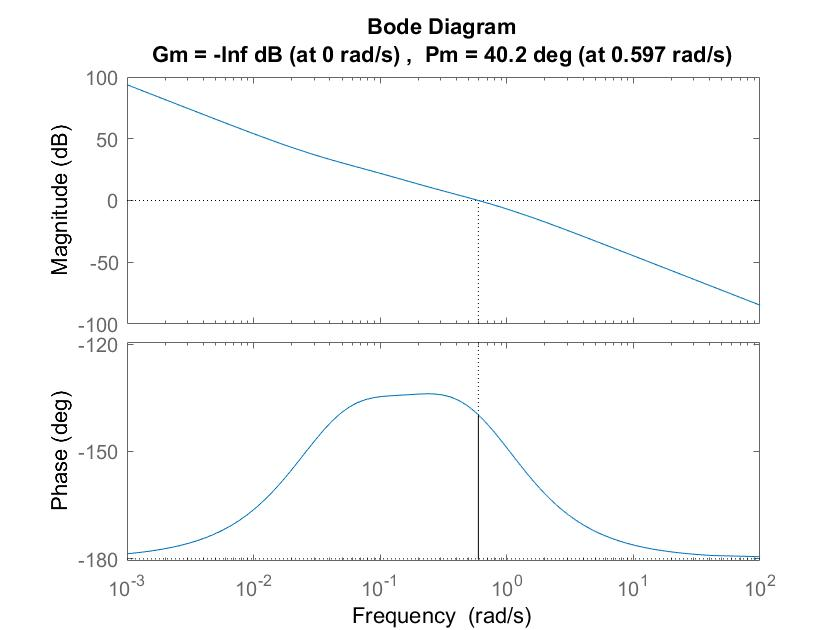
\includegraphics[scale = 0.4]
{L2_PI_Bode}
\caption{Bode plot of the open F2-L2 loop with PI control}
\label{PI_bode}
\end{figure}

\begin{figure} [H]
\centering	\includegraphics[scale = 0.6]{PI_set}
\caption{Response of the L2-F2 control loop with PI control}
\label{PI_set}
\end{figure}

\begin{figure} [H]
\centering	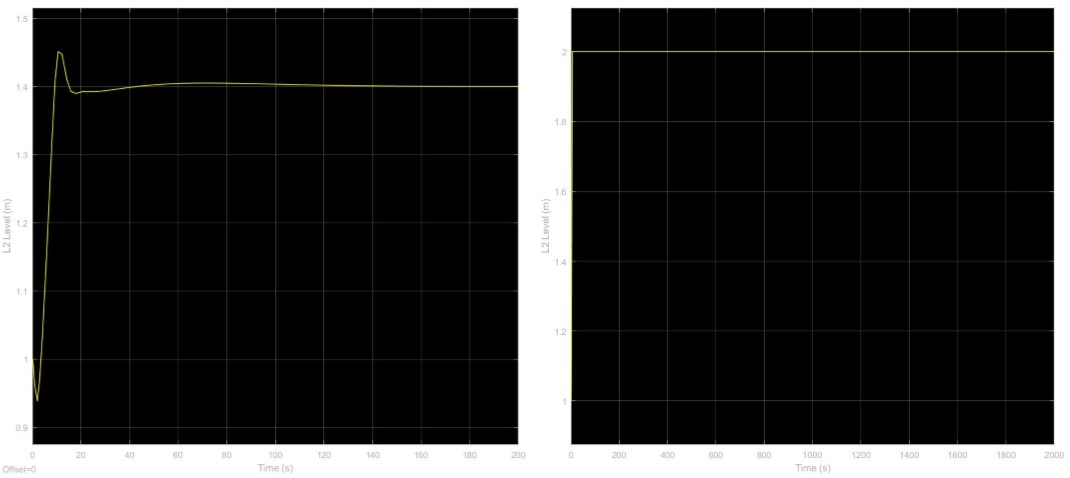
\includegraphics[scale = 0.6]
{X2_levels}
\caption{Response of the L2-F2 control loop with PI control for X1 at 0\% (Left) and 40\% (Right)}
\label{X2_Levels}
\end{figure}

\begin{figure} [H]
\centering	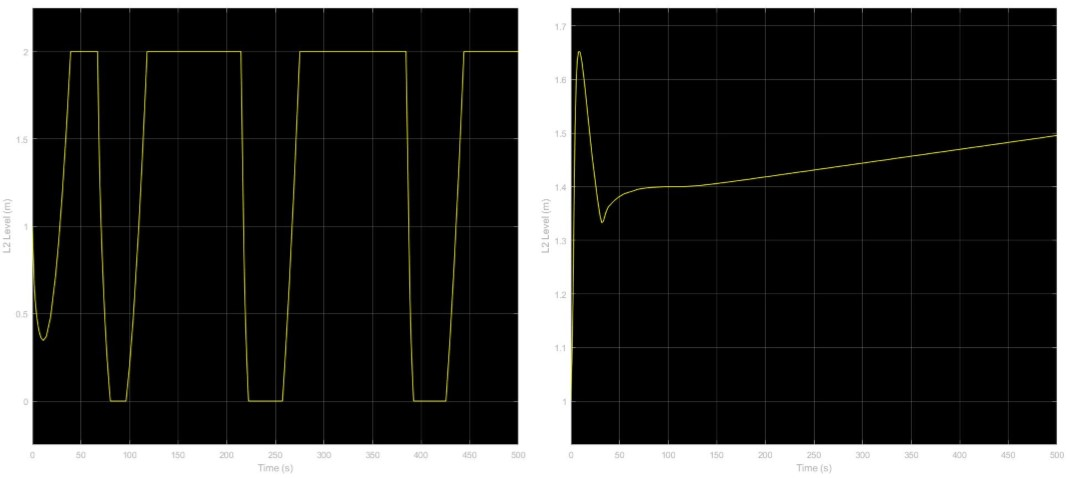
\includegraphics[scale = 0.6]
{F2_levels}
\caption{Response of the L2-F2 control loop with PI control for F1 at 7kg/min (Left) and 12.32kg/min (Right)}
\label{F2_Levels}
\end{figure}

\subsubsection{Simulink Models}
\begin{figure} [H]
\centering	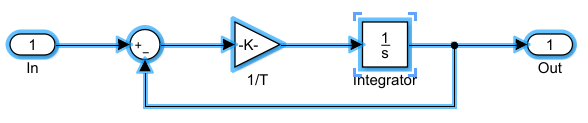
\includegraphics[scale = 0.5]
{servo}
\caption{Model of the delay caused by the servos}
\label{F2_Levels}
\end{figure}

\begin{figure} [H]
\centering	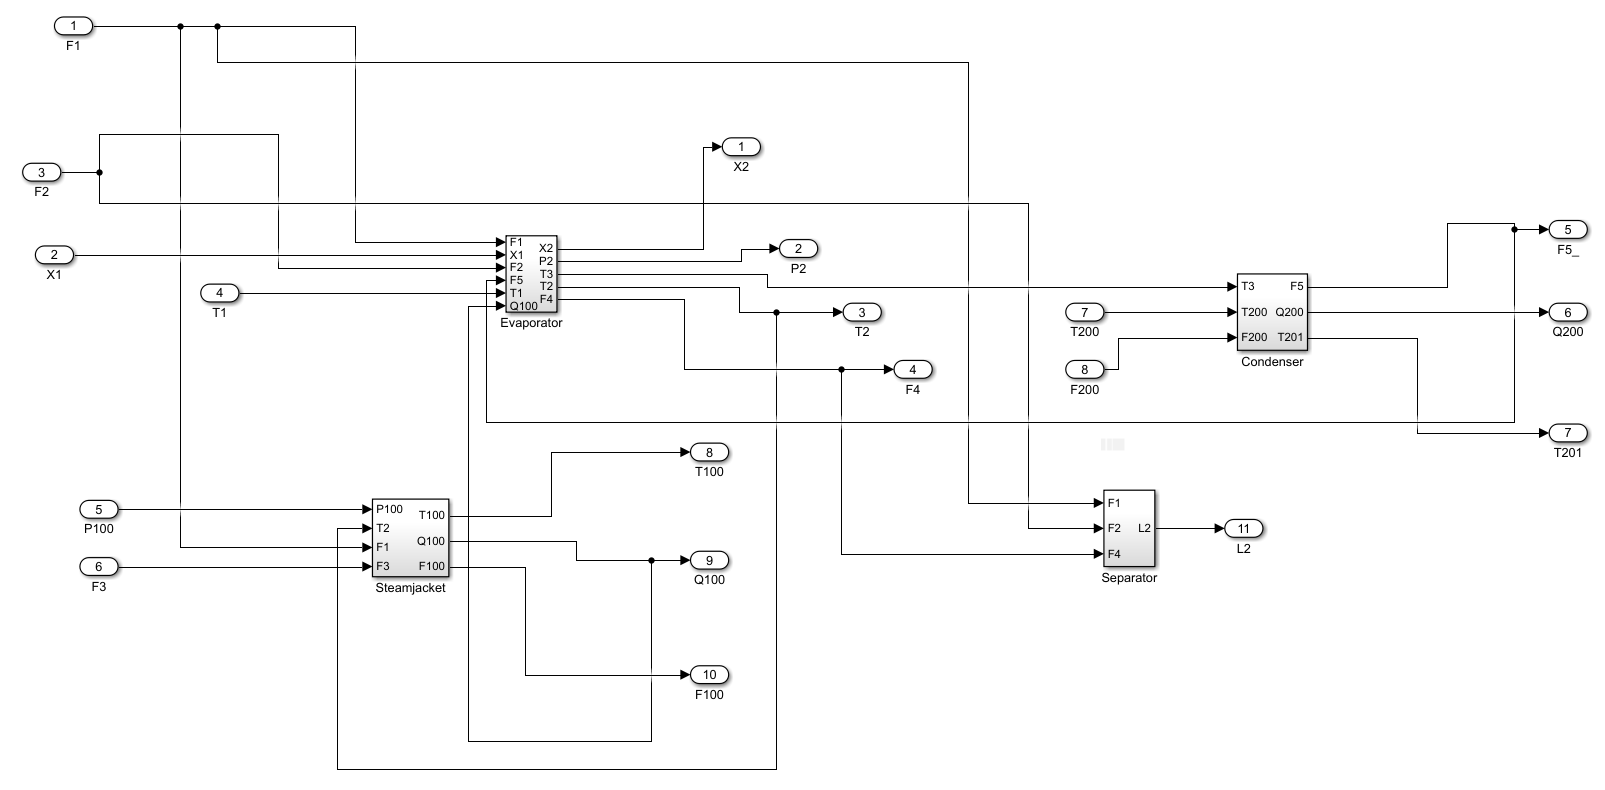
\includegraphics[scale = 0.5]{process}
\caption{Model of the process at nominal values with servos and L2-F2 control}
\label{F2_Levels}
\end{figure}

\end{document}